\documentclass[10pt]{article}
\usepackage[margin=0.5in]{geometry}
\usepackage{titling}
\usepackage[compact]{titlesec}
\usepackage{url}
\usepackage{fontspec}
\usepackage{graphicx}
\usepackage{float}

\setlength{\droptitle}{-4em}
\addtolength{\droptitle}{-4pt}

\title{Embedded System Design \\ Traffic Light}
\author{ Max Thrun | Ian Cathey | Mark Labbato }

\begin{document}
\maketitle

\section*{Abstract}

The purpose of this project was to simulate traffic lights at an intersection
which is controlled by software and use priorities to tell the operating
system how to schedule the different tasks.

\section*{Implementation / Design}

The first step we took in implementing our project was to break down the
functionality of the intersection and figure out the priority of each function.
We ended up matching the assignment document exactly in terms of functionality
per task and priority of each task. We determined task A to be the lowest
priority and each following task to be a higher priority than the previous all
the way up to the highest priority task, task F. In regards to the length of
each light we did not want to use \emph{actual} intersection timing as it would
take for ever to test. We therefore used what we felt were accurate
\emph{relative} timings. For instance the primary street green is twice as long
as the secondary street green. It really does not matter what the timings are
as we are more concerned with sequencing and event control. 
\\\\
Our next design decision was how to display the status of the intersection and
how we would control events such as a car being in the turning lane or the walk
button being pressed. After evaluating all the IO on the DE1 we decided that
the cleanest and clearest way to convey all this information would be to
utilize the JTAG UART functionality of the Nios 2 and actually draw the
intersection in the terminal using ANSI control sequences to set color and
position of different things such as the lights and cars in the turn lane. This
allows us to see the whole state of our intersection without trying to have to
decode LED sequences or 7-segment characters on the DE1 board. Additionally, we
can use the receiving side of the JTAG UART to read characters from the
keyboard on the PC.  This allows us to logically map keys such as 'w' to the
walk button. We found this to be a much cleaner solution that trying to
remember which switch or button on the DE1 corresponded to which functionality.
\\\\ 
Once our IO functionality was decided, the first step was to write
thread-safe drawing functions to draw things to the terminal such as the lanes
of the street and the lights at the proper position and color. Thread-safety
was achieved by a `draw\_lock' mutex which each drawing function waits to
obtain before writing anything to the UART. This ensures that two threads wont
interrupt each other when trying to update the screen. To read bytes off the
UART a separate task is used which actually has the highest priority in our
whole program. This task continuously calls getc() to try and read the next
byte in the UART buffer and if a byte is read it uses its value to set a flag in a
global `key\_down' array.  For instance, if the key 'a' is pressed, which has
an ASCII value of 97, then key\_down[97] is set to 1. A seperate function
called `key\_pressed(char key)` is used to check if a ceratin key has been
pressed. For instance, calling `key\_pressed('w')' will check the key\_down[]
array to see if key\_down['w'] is set to a 1. If it is set it will clear it to
a 0, since it's now been handled, and return true. The key\_down array is
protected by a 'input\_lock' mutex to avoid reading and writing at the same
time.  
\\\\ After establishing all the IO routines we were able to quickly
implement each task.  In order to keep a modular design each task is
independent in the sense that when that task is running it does not depend on
any other task to control the lights.  A global mutex called 'light\_lock' is
used to control which task is controlling the lights. A task must acquire this
mutex before attempting to modify the light values. This works well because it
ensures that higher priority tasks will always gain control of the lights when
they need it. Each task, except for manual mode task F, keeps track A what it
is currently doing by using a state machine. This is an ideal control scheme
for this project because the nature of a traffic light can be viewed as a state
machine. For instance, in task A, a switch case is used to go from Primary
Green, to Primary Yellow, to Primary Red, etc... In the other tasks there is an
initial state which just waits for input such as the walk button being pressed.
Once the walk button is pressed it goes to the next state which waits for all
lights to turn red. It then goes to the next state which locks the lights and
makes the walk light green. It then goes the to next state which makes it
yellow, etc.. It's easy to see how using state machines allows the required
sequential functionality to be directly implemented.

\newpage
\section*{Program Output}
The terminal output showing an `ASCII art' representation of the intersection
is shown below. Using Unicode characters allowed us to draw nice continuous
lines, corners, and arrows. ANSI control sequences allowed us to achieve proper
colors for the lanes and lights. The top right section shows the key mapping to
control the functionality of the intersection and the bottom right section
shows status and debug output describing the current state of the intersection.
The blue squares in the primary street turn lanes indicate a car is waiting.

\begin{figure}[H]
    \centering
    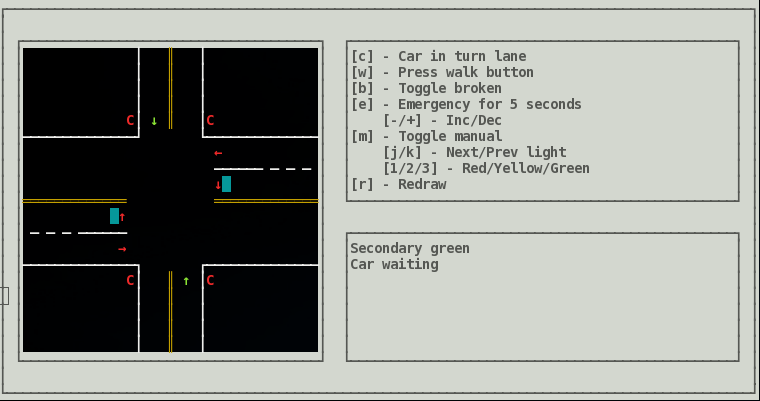
\includegraphics[width=0.6\textwidth]{lights.png}
    \caption{Terminal Output}
\end{figure}

%\begingroup
%\setmonofont{DejaVu Sans Mono}
%\begin{center}
%\begin{tiny}
%\begin{verbatim}
%┌─────────────────────────────────────────────────────────────────────────────────────────────┐
%│                                                                                             │
%│ ┌─────────────────────────────────────┐  ┌────────────────────────────────────────────────┐ │
%│ │              │   ║   │              │  │[c] - Car in turn lane                          │ │
%│ │              │   ║   │              │  │[w] - Press walk button                         │ │
%│ │              │   ║   │              │  │[b] - Toggle broken                             │ │
%│ │              │   ║   │              │  │[e] - Emergency for 5 seconds                   │ │
%│ │             C│ ↓ ║   │C             │  │    [-/+] - Inc/Dec                             │ │
%│ │──────────────┘       └──────────────│  │[m] - Toggle manual                             │ │
%│ │                        ←            │  │    [j/k] - Next/Prev light                     │ │
%│ │                        ────── ─ ─ ─ │  │    [1/2/3] - Red/Yellow/Green                  │ │
%│ │                        ↓            │  │[r] - Redraw                                    │ │
%│ │═════════════           ═════════════│  └────────────────────────────────────────────────┘ │
%│ │            ↑                        │                                                     │
%│ │ ─ ─ ─ ──────                        │  ┌────────────────────────────────────────────────┐ │
%│ │            →                        │  │Primary green                                   │ │
%│ │──────────────┐       ┌──────────────│  │                                                │ │
%│ │             C│   ║ ↑ │C             │  │                                                │ │
%│ │              │   ║   │              │  │                                                │ │
%│ │              │   ║   │              │  │                                                │ │
%│ │              │   ║   │              │  │                                                │ │
%│ │              │   ║   │              │  │                                                │ │
%│ └─────────────────────────────────────┘  └────────────────────────────────────────────────┘ │
%│                                                                                             │
%└─────────────────────────────────────────────────────────────────────────────────────────────┘
%\end{verbatim}
%\end{tiny}
%\end{center}
%\endgroup


\section*{Testing Strategy}
Given the modular approach of our design testing the functionality of each task
was extremely easy.  We were able to develop each task in parallel and test
their individual functionality independently.  The only exception to this is
task A, which a few other tasks depend on. For instance, task b waits until the
primary street is about to turn green and task c waits until all lights are
red. Overall the testing and integrating of each task went flawlessly which we
attribute mostly to our choice in IO. We were, at a glance, able to see the
entire state of our system and quickly test out the different inputs without
having to remember if switch 1 was for the walk button or emergency. Had we
chosen to use LEDs and switches we might not have had this advantage.

\section*{Implementation Resource Usage}
Using the 'nios2-elf-size' command we can get a breakdown of our programs resource utilization
\begin{enumerate}
    \item[]
\begin{verbatim}
$ nios2-elf-size traffic.elf 
   textwidth   data    bss    Dec    hexfilename
      105580   7044  71332 183956  2ce94traffic.elf
\end{verbatim}
\end{enumerate}
The Quartus build summary provides a summary of the FPGA utilization.
\begin{enumerate}
\item[]
\begin{verbatim}
Fitter Status : Successful - Mon Nov 26 20:51:57 2012
Quartus II 32-bit Version : 12.0 Build 178 05/31/2012 SJ Web Edition
Revision Name : top
Top-level Entity Name : top
Family : Cyclone II
Device : EP2C20F484C7
Timing Models : Final
Total logic elements : 2,832 / 18,752 ( 15 % )
    Total combinational functions : 2,366 / 18,752 ( 13 % )
    Dedicated logic registers : 1,861 / 18,752 ( 10 % )
Total registers : 1929
Total pins : 80 / 315 ( 25 % )
Total virtual pins : 0
Total memory bits : 44,032 / 239,616 ( 18 % )
Embedded Multiplier 9-bit elements : 0 / 52 ( 0 % )
Total PLLs : 1 / 4 ( 25 % )
\end{verbatim}
\end{enumerate}
\section*{Implementation Speed and Power}
The max clock speeds as indicated by the Timing Analyzer is shown below
\begin{enumerate}
    \item[]
        \begin{verbatim}
+------------------------------------------------------------------+
; Slow Model Fmax Summary                                          ;                                                                                                                                                                                    
+------------+-----------------+----------------------------+------+
; Fmax       ; Restricted Fmax ; Clock Name                 ; Note ;
+------------+-----------------+----------------------------+------+
; 80.33 MHz  ; 80.33 MHz       ; u0|altpll_0|sd1|pll|clk[0] ;      ;
; 252.91 MHz ; 252.91 MHz      ; u0|altpll_0|sd1|pll|clk[2] ;      ;
+------------+-----------------+----------------------------+------+
\end{verbatim}
\end{enumerate}
The thermal power dissipation as indicated by Power Play is shown below
\begin{enumerate}
    \item[]
        \begin{verbatim}
PowerPlay Power Analyzer Status : Successful - Sun Dec  9 21:50:01 2012
Quartus II 32-bit Version : 12.0 Build 178 05/31/2012 SJ Web Edition
Revision Name : top
Top-level Entity Name : top
Family : Cyclone II
Device : EP2C20F484C7
Power Models : Final
Total Thermal Power Dissipation : 149.99 mW
Core Dynamic Thermal Power Dissipation : 48.74 mW
Core Static Thermal Power Dissipation : 47.50 mW
I/O Thermal Power Dissipation : 53.75 mW
Power Estimation Confidence : Low: user provided insufficient toggle rate data
        \end{verbatim}
\end{enumerate}
Our critical path seems to be the interface with the SDRAM as shown by the Timing Analyzer
\begin{enumerate}
    \item[]
        \begin{verbatim}
+-------------------------------------------------------------------------------------------
; Fast Model Setup: 'u0|altpll_0|sd1|pll|clk[0]'                                            
+--------+----------------------------------------------------------------------------------
; Slack  ; From Node                                                                        
+--------+----------------------------------------------------------------------------------
; 15.098 ; nios_system:u0|nios_system_sdram_0:sdram_0|nios_system_sdram_0_input_efifo_module
; 15.127 ; nios_system:u0|nios_system_sdram_0:sdram_0|nios_system_sdram_0_input_efifo_module
; 15.167 ; nios_system:u0|nios_system_sdram_0:sdram_0|nios_system_sdram_0_input_efifo_module
; 15.182 ; nios_system:u0|nios_system_sdram_0:sdram_0|nios_system_sdram_0_input_efifo_module
...
        \end{verbatim}
\end{enumerate}

\section*{Team Member Contributions}
\begin{itemize}
    \item \textbf{Max Thrun} - Print/drawing functions, UART input task, task F
    \item \textbf{Ian Cathey} - Task A, Task C, Task D
    \item \textbf{Mark Labatto} - Task B, Task E, Task D
\end{itemize}
\end{document}
